\chapter{Einleitung}

% problemstellung
% ziele definieren
% vorhandene daten beschreiben
\section{Problemstellung}
% - Ausschneiden von Fotos aus einem Fotoalbum \\
% - Fotoalbumseite sauber eingescannt \\
% - Bilder mit Rahmen, der entfernt werden soll \\
% - Gesichtserkennung mit Ausschneiden der Gesichter \\
% - Seite eines Fotoalbums besteht aus Hintergrund und eingeklebten Fotos \\
% - Einfaches modulares Programm ohne grafische Oberfläche \\
% - Erstellen von Metriken um die Ergebnisse zu überprüfen

Die hier entwickelte Software soll aus einer eingescannten Fotoalbumseite die darin enthaltenen Fotos extrahieren. Dazu sollte die Seite des Fotoalbums sauber eingescannt sein mit einem möglichst gleichfarbigen Hintergrund und ohne Spiegelungen. Die Fotos können einen Rahmen haben, der von dem Programm entfernt wird.
Sobald die Fotos ausgeschnittenen wurden kann für jedes einzelne Foto innerhalb der Fotoalbumseite eine Gesichtserkennung durchgeführt werden, bei der die erkannten Gesichter markiert und ausgeschnitten werden.
Um das Ergebnis der Software zu überprüfen soll es möglich sein die ausgeschnittenen Fotos mit Ground Truth Bildern auf Ähnlichkeit zu vergleichen. Das Programm soll über die Kommandozeile ausgeführt werden und in einzelne Module aufgeteilt sein, sodass einzelne Elemente jeder Zeit angepasst werden können.
 
\section{Benutzte Technologien}
% genutzte methoden, toolboxen, programmiersprachen
Für die Entwicklung dieser Software wurde als Programmiersprache Python 3.6 verwendet zusammen mit der Bibliothek numpy in der Version 1.14.2. Numpy ermöglicht die schnellere Berechnung von Matrizen und wird für die Bibliothek OpenCV in der Version 3.4.0.12 benötigt. OpenCV bietet eine reihe von Algorithmen für die Bildbearbeitung. Um eine Auswertung anzufertigen wurde aus der Bibliothek SciKit-image 0.13.1 die Methode zur Berechnung der strukturellen Ähnlichkeit (SSIM) verwendet.

\section{Programmaufbau}
Das Programm teilt sich in fünf Hauptkomponenten auf. Die erste ist in der \textit{main.py} zu finden, die das Programm startet und die anderen Komponenten ausführt. Die zweite Komponente kümmert sich um das entfernen des allgemeinen Hintergrunds und ist in der \textit{backgroundremover.py} zu finden. In dieser Komponente werden die eigentlichen Fotos aus dem Fotoalbum grob ausgeschnitten. Danach wird in der nächsten Komponente für jedes Foto der Rahmen entfernt, falls ein Rahmen vorhanden ist. Das entfernen des Rahmens geschieht in der \textit{rectextract.py}. Die letzte Komponente ermöglicht es Gesichter in den ausgeschnittenen Bildern zu erkenne. Dies geschieht in der \textit{facedetection.py}. Möchte man die ausgeschnittenen Bilder mit Beispielbildern vergleichen, so kann man die letzte Komponente in der Datei \textit{compare.py} verwenden. Mit deren Hilfe Metriken aufgestellt werden zum Vergleich der Bilder. In dem Flussdiagramm \ref{fig:flowchart} ist der Ablauf des Programmes nochmals genauer als Diagramm dargestellt.

\begin{figure}[h]
	\centering
	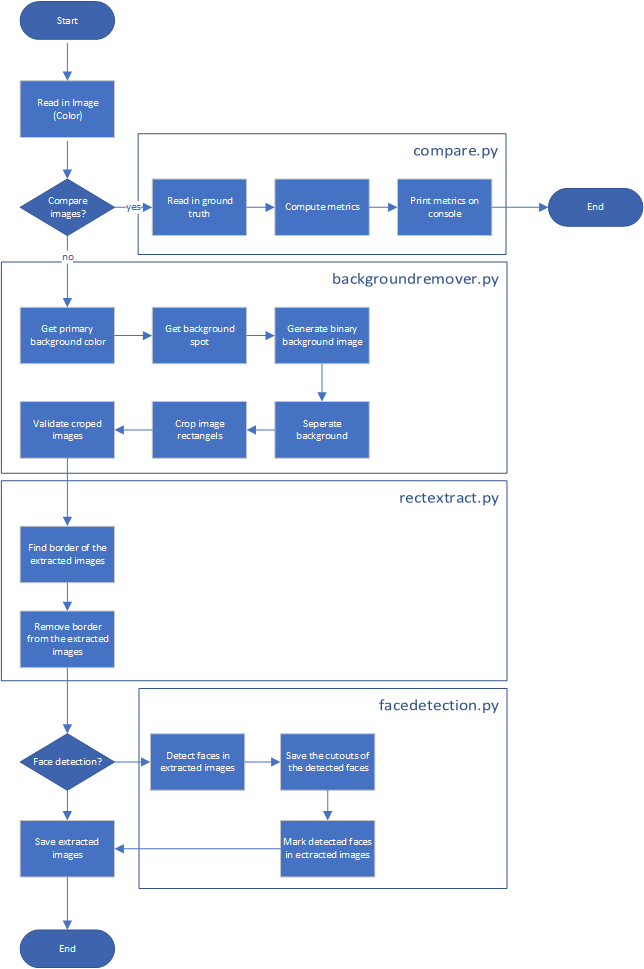
\includegraphics[width=0.45\linewidth]{images/flowchart.png}
	\caption{Flussdiagramm, das den Ablauf des Programmes darstellt. Verzweigungen können mit Hilfe von Parametern bei der Ausführung des Programmes gesteuert werden.}
	\label{fig:flowchart}
\end{figure}
